\section{Aufbau und Durchführung}

\subsection{Aufbau}
Der Aufbau des Versuches ist relativ simpel (\ref{fig:1}) . Auf der einen Seite befindet sich die Strahlungsquelle, in unserem
Fall Cs-137, welches von großes Bleiböcken abgeschirmt wird, sodass ein schmaler Strahl entsteht. Gegenüber 
von der Quelle befindet sich ein NaJ-Detektor. Mit diesem wird die $\gamma$-Strahlung detektiert. 

\noindent
Unterhalb des Strahlengangs befindet sich eine Platte, auf welche sich Proben montieren lassen. Diese lässt 
sich verschieben und drehen. Im Versuch wurden auf dieser mehrere Würfel platziert. 2 waren gefüllt mit einem
umbekannten Metall, einer war leer (für eine Referenzmessung) und einer war gefüllt mit 27 kleineren Würfeln
, welche das Volumen des großen Würfels füllen.

\begin{figure}[H]
	\centering
	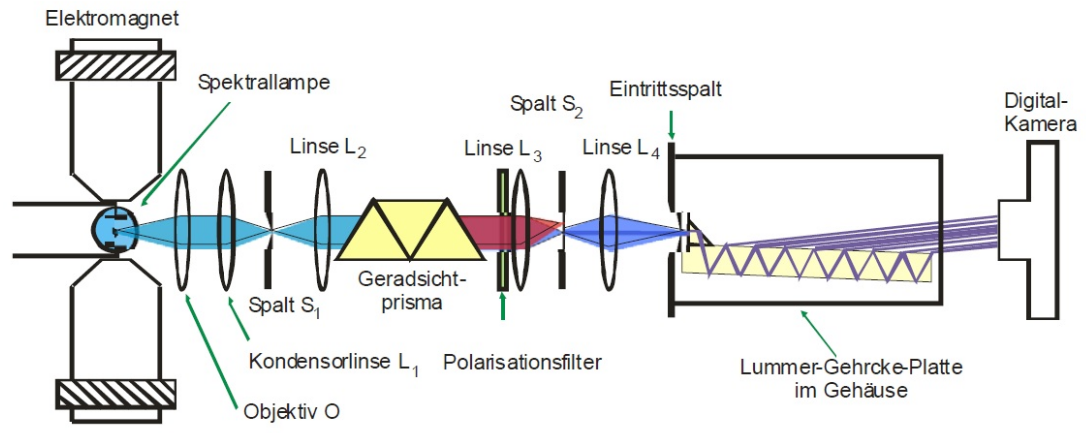
\includegraphics{aufbau.png}
	\caption{Foto vom Aufbau des Experimentes \biber}
	\label{fig:1}
\end{figure}

\noindent
Da die Platte nicht in der Höhe verstellbar war wurde lediglich die 2. Schicht des Würfels gemessen, sodass nur eine Bestimmung von 9 kleineren Würfeln möglich war. Der Aufbau ist
in der \autoref{fig:aufbau} dargestellt.

\begin{figure}
    \centering
    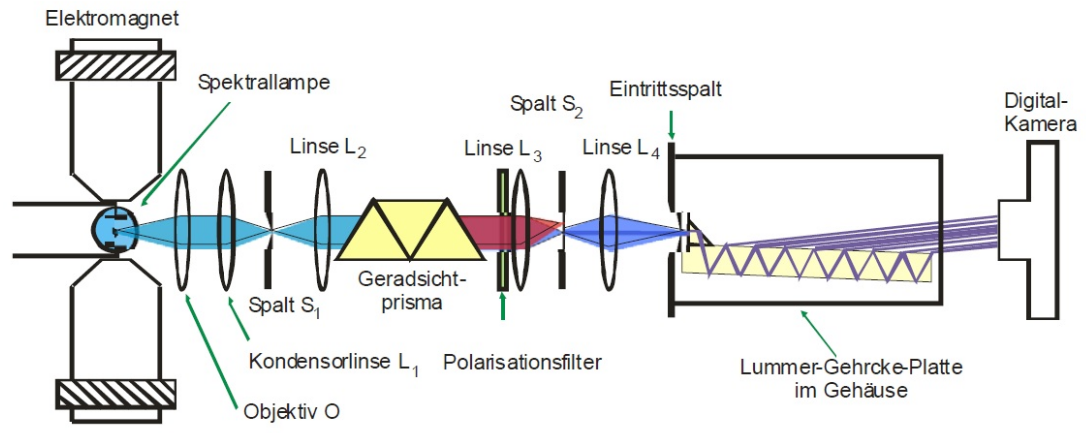
\includegraphics[width=0.75\textwidth]{aufbau.png}
    \caption{Versuchsaufbau \cite{V14}}
    \label{fig:aufbau}
  \end{figure}

\noindent
Als mögliche Stoffe kommen nur Aluminium, Blei, Eisen, Messing ($Cu_{0.63}Zn_{0.37}$) und Delrim (POM) infrage \cite{V14}. 

\noindent
Als zusätzliche Aufbautewird  ein Multichannelanalyzer (kurz MCA) genutzt. Mithilfe diesem werden elektrische Impulse mit unterscheidlichen Aplituden ihrer Häufigkeit nach sotieren. 

\subsection{Szintillationsdetektor}
Mithilfe eines Szintillationsdetektors kann die Energie und Intensität von ionisierender Strahlung bestimmt werden. Dieser kann aus organischen, aber auch aus anorganischen Stoffen
bestehen. Der im Versuchsaufbau verwendete Szintillationsdetektor nutzt einen anorganischen Natriumiodidkristall, welcher, wenn eine Energie größer als die Anregungsenergie 
dessen in ihn eindringt, sogenannte 'Lichtblitze' erzeugt, die durch einen Bandwechsel von angeregten Elektronen entstehen. Die freigesetzten Photonen werden mithilfe eines 
Photomultipliers detektiert. Der Strom der in dem Photomultiplier entsteht ist propotional zu der Energie des $\gamma$-Quants, welches für die Erzeugung des detektierten Photons
durch den Photomultiplier verantwortlich ist. 


\subsection{Durchführung}
Zur Hilfe mit der Messung wird das Programm MAESTRO genutzt.

\noindent
Zuerst wird ein Spektrum der verwendeten Quelle genutzt. Gemessen wird solange bis mindestens am Peak 1112 Impulse gemessen wurden. Da ein relative Unsicherheit < 0,03
gewünscht ist und kann mithilfe des Zusammenhangs

\begin{equation}
    \frac{\sqrt{N}}{N} = 0,03 \leftrightarrow N = \frac{1}{0,03^2} \approx 1112
    \label{eqn:n}
  \end{equation}
  
die Mindestanzahl an Peaks so ermittelt werden. Das Programm zeigt dies an, sodass einfach die Messung auf ein USB Stick expotiert werden können.

\noindent
Bei dem leeren Würfel, dem 2 Würfel und dem 3x3x3 Würfel wurden alle Strahlengänge nach der \autoref{fig:projektion} gemessen. Beim 3. Würfel wurden lediglich die Strahlengänge
1,2,3,10,11,12 gemessen. 

\noindent
Da das Programm automatisch nach 300s aufhört musste bei dem 3. Würfel der Strahlengang 11 und beim 3x3 Würfel der Strahlengang 8 und 11 2 mal gemessen und später in der
Auswertung addiert werden, um die Messunsicherheiten gering zu halten.












